 \documentclass[h]{article}
\usepackage[margin=0.5in]{geometry}
\usepackage{amsfonts} 
\usepackage{textcomp}
 
\usepackage{graphicx}
\usepackage{caption}
\usepackage{subcaption}
\usepackage{float} 
\usepackage{flafter}
\graphicspath{ {./plots/} }
\usepackage{adjustbox}


\newcommand{\cent}{\textcent \hspace{4pt}}
\title{CS 7641 Machine Learning \\ Assignment 3}
\date{Due Sunday April 1st, 2018 11:59pm}
\author{Philip Bale \\ pbale3}

\begin{document}

\maketitle

\section*{Introduction}  
This assignment explores unsupervised learning and dimensitonality reduction.  
It begins by examining clustering algorithms, specifically k-means and 
expectation maximization.  It then proceeds to cover four dimensionality 
reduction algorithms: principal components analysis, individual components 
analysis, randomized projections, and random forests.  After running these six 
algorithms on the original datasets and observing the results, the results are 
then piped into a neural network learner for further examination.

\subsection*{Datasets chosen}  
The datasets chosen were the same datasets chosen for assignment 1.  The first dataset is the US 
permanent visa dataset.  This dataset is interesting due to its potential to aid in the visa application process 
from a cost and time savings potential. It could also enable confidence in those interested in applying for a 
US permanent visa but doubting their chances of acceptance. 
At the end of the day, the goal is it to try to determine the application result before time, money, 
nd other resources are spent. 
\\  \\
The second dataset is a home sale price prediction dataset taken from an ongoing 
Kaggle competiton.  This dataset is interesting for two primary reasons: real-world applicability and participating in a Kaggle challenge.
 First, modeling home prices is both a difficult and lucrative task. 
 If one can succesfully model home sale prices on large sets of data, he/she can make large amounts of money 
 investing in real estate when he/she detects outliers in listed price vs. what it is expected to sell for. 
 This applies to flipping, investing, and remodeling. 
 Second, the dataset is part of an ongoing Kaggle competition that does not have a winning solution yet.
  By taking part of the competition, the dataset presents the opportunity to work towards a winning solution 
  and advance ones algorithms over time.

\section*{Part 1: Clustering Algorithms}
\subsection*{Introduction}  
K-means clustering is the first algorithm applied to the datasets and expectation maximization is the second. 
 Both algorithms work by clustering: gathering groups of instances together 
 based upon their features.  The rationale is that similar instances will likely 
 be labeled the same way--such as identical visa applications obtaining the same 
 outcome.

\subsection*{1) k-means clustering}  
\subsubsection*{Overview}
K-means works by clustering n instances into k-clusters of similarity using least-squares Euclidean distance
 between the instances.  In practice, the algorithm converges on 'mean' for each cluster that is representative of the 
 members of that cluster.   A variety of cluster sizes were tested to find the best parameters 
 possible.
 
 \begin{figure}[H]
  \minipage{0.33\textwidth}
      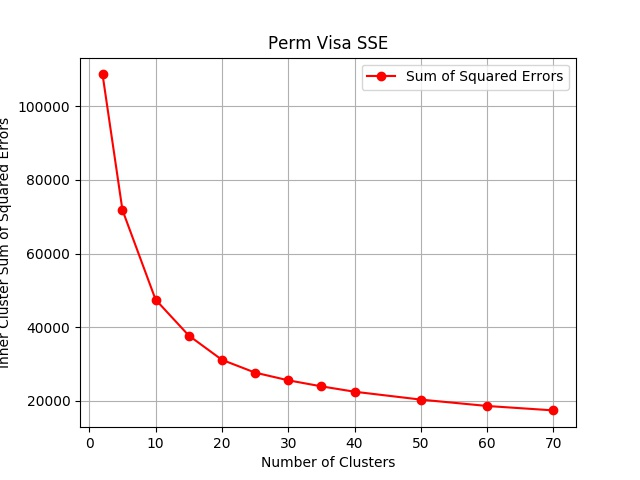
\includegraphics[width=1\textwidth,keepaspectratio]{perm_visa_sse.jpg} 
      \caption*{Perm Visa Sum of Square Errors for Clusters vs. \# Clusters} 
   \endminipage\hfill
      \minipage{0.33\textwidth}
      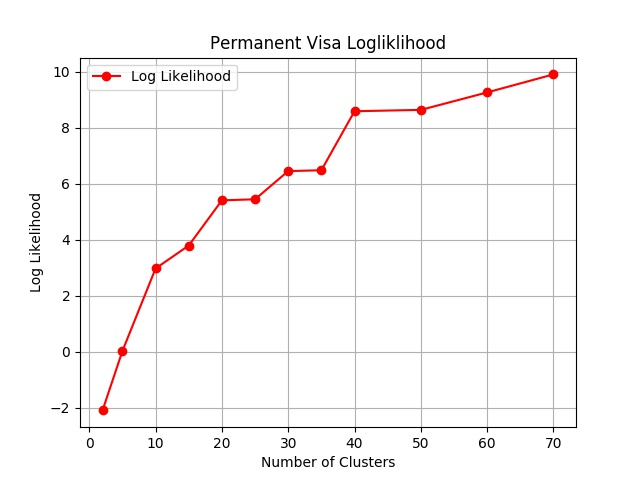
\includegraphics[width=1\textwidth,keepaspectratio]{permanent_visa_logliklihood.jpg} 
      \caption*{Perm Visa Log Liklihood vs. \# Components} 
   \endminipage\hfill
   \minipage{0.33\textwidth}
      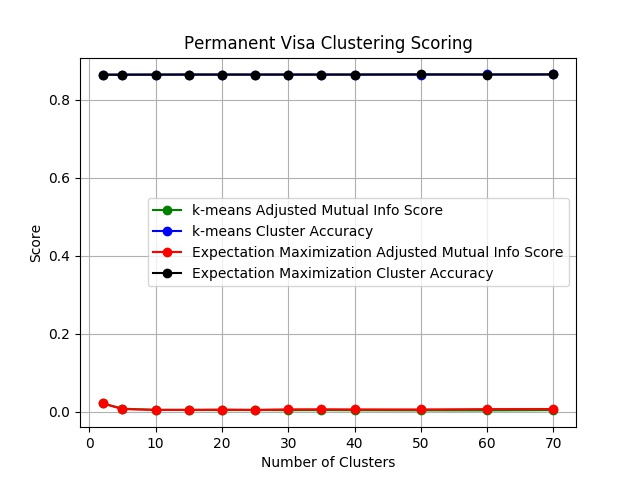
\includegraphics[width=1\textwidth,keepaspectratio]{permanent_visa_clustering_scoring.jpg} 
      \caption*{Perm Visa Scoring for k-means and expectation maximization} 
   \endminipage\hfill
\end{figure}
 \begin{figure}[H]
  \minipage{0.33\textwidth}
      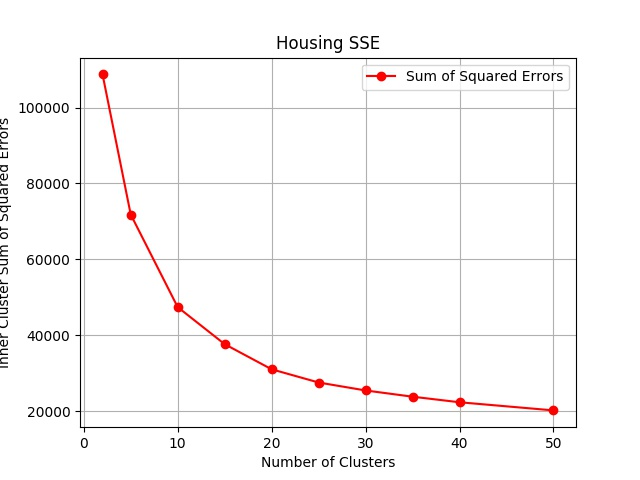
\includegraphics[width=1\textwidth,keepaspectratio]{housing_sse.jpg} 
      \caption*{Housing Sum of Square Errors for Clusters vs. \# Clusters} 
   \endminipage\hfill
   \minipage{0.33\textwidth}
      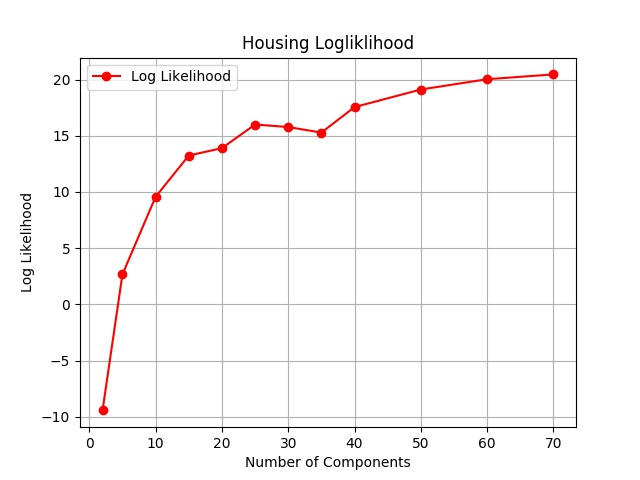
\includegraphics[width=1\textwidth,keepaspectratio]{housing_logliklihood.jpg} 
      \caption*{Housing Log Liklihood vs. \# Components} 
   \endminipage\hfill
   \minipage{0.33\textwidth}
      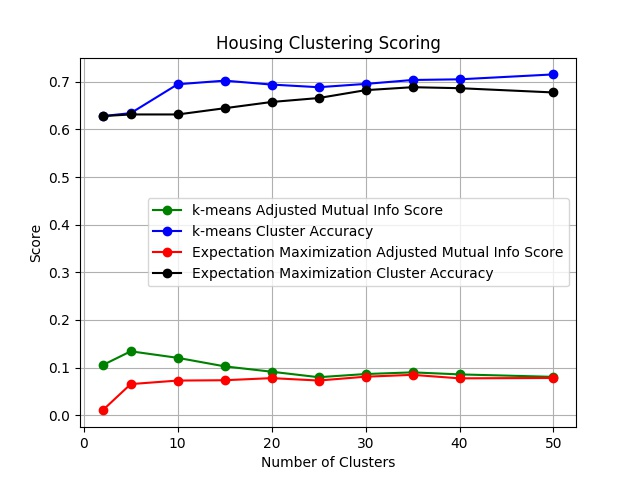
\includegraphics[width=1\textwidth,keepaspectratio]{housing_clustering_scoring.jpg} 
      \caption*{Housing Scoring for k-means and expectation maximization} 
   \endminipage\hfill
\end{figure}

\subsubsection*{k-Means Analysis}
Text

\begin{figure}[H] 
\begin{tabular}{ | c | c  | c | c | c | c | c | c| c| c| c| c| c | } 
\hline
\textbf{ # Clusters } & \textbf{2} & \textbf{5} & \textbf{10} & \textbf{15} & \textbf{20} & \textbf{25} & \textbf{30} & \textbf{35} & \textbf{40} & \textbf{50} & \textbf{60} & \textbf{70}   \\
\hline
\textbf{PERM VISA} \\ \hline
\textbf{SSE} &  108717 & 71834 & 47453 & 37701 & 31090 & 27611 & 25517 & 23874 & 22410 & 20267 & 18532 & 17331 \\ \hline
\textbf{Log Liklihood} & -9.44 & 2.67 & 9.57 & 13.25 & 13.90 & 16.01 & 15.78 & 15.29 & 17.56 & 19.12 & 20.04 & 20.47 \\ \hline
\textbf{k-Means AMI} & 0.022 & 0.008 & 0.005 & 0.005 & 0.004 & 0.005 & 0.004 & 0.004 & 0.004 & 0.004 & 0.004 & 0.004 \\ \hline
\textbf{k-Means ACC} & 0.865 & 0.865 & 0.865 & 0.865 & 0.865 & 0.865 & 0.865 & 0.865 & 0.865 & 0.865 & 0.865 & 0.865 \\ \hline
\textbf{EM AMI} & 0.022 & 0.007 & 0.005 & 0.005 & 0.006 & 0.005 & 0.006 & 0.007 & 0.006 & 0.006 & 0.007 & 0.007 \\ \hline
\textbf{EM ACC} & 0.865 & 0.865 & 0.865 & 0.865 & 0.865 & 0.865 & 0.865 & 0.865 & 0.865 & 0.865 & 0.865 & 0.865 \\ \hline
\\
\textbf{HOUSING} \\ \hline
\textbf{SSE} & 14840 & 10217 & 8265 & 7256 & 6589 & 6106 & 5687 & 5339 & 5063 & 4589 & 4276 & 4024 \\ \hline
\textbf{k-Means AMI} & 0.105 & 0.134 & 0.120 & 0.103 & 0.091 & 0.080 & 0.086 & 0.090 & 0.086 & 0.081 & 0.083 & 0.081 \\ \hline
\textbf{k-Means ACC} & 0.628 & 0.634 & 0.695 & 0.702 & 0.694 & 0.688 & 0.695 & 0.704 & 0.705 & 0.715 & 0.719 & 0.726 \\ \hline
\textbf{EM AMI} & 0.010 & 0.065 & 0.073 & 0.073 & 0.078 & 0.073 & 0.081 & 0.085 & 0.077 & 0.078 & 0.065 & 0.064 \\ \hline
\textbf{EM ACC} & 0.628 & 0.631 & 0.631 & 0.644 & 0.657 & 0.666 & 0.682 & 0.688 & 0.686 & 0.677 & 0.673 & 0.679 \\ \hline
\end{tabular}
\caption*{Table of Housing Data Results for Cluster } 
\end{figure}

\subsection*{2) Expectation Maximization}  
\subsubsection*{Overview}
Expectation Maximization is the second algorithm applied to the datasets and, 
similar to k-means, is a clustering algorithm.  Expectation Maximization works 
by iteratively finding the maximum liklihood of parameters leading to a labeling 
of an instance despite possibly not having all data or parameters.  For our 
examples, we used Scikit-learn's Gaussian mixture models to implement the 
Expectation Maximization algorithm.  A varying number of mixture components (or number of distributions) were 
used to determine the best possible parameters for the clustering.

\subsubsection*{Expectation Maximization Analysis}
Text








 
\section*{Part 2: Dimensionality Reduction Algorithms}
\subsection*{ Introduction}  
Part 2 deals with dimensionality reduction algorithms.  The four algorithms used 
are principal components analysis, individual components analysis, randomized projections, and random 
forests.  After running the algorithms on both datasets, an analysis is provided 
on the results.

\subsection*{1) Principal Components Analysis (PCA)}  
\subsubsection*{Overview}
The first dimenstionality reductation algorithm, Principal component analysis is a statistics approach to finding vectors that 
maximize variance and thus help to determine components that are correlated.  Each subsequent component is found with the intent to be 
orthoganal to the preceding component.  The resulting eigenvalue matrix from PCA 
is therefore maximized for covariance.

 \begin{figure}[H]
  \minipage{0.49\textwidth}
      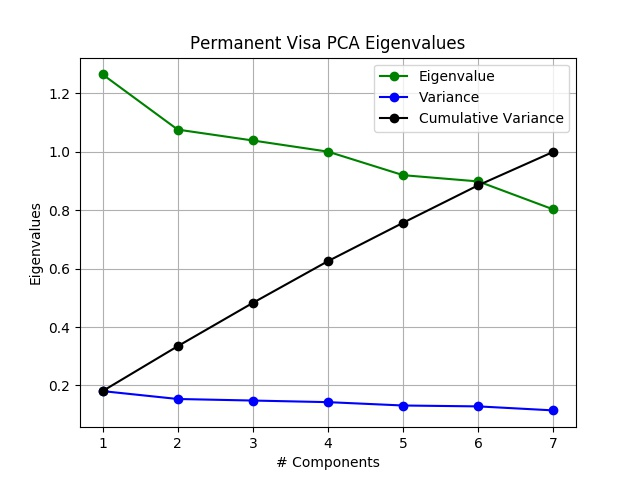
\includegraphics[width=1\textwidth,keepaspectratio]{permanent_visa_pca_eigenvalues.jpg} 
      \caption*{Permanent Visa Principal Components Analysis } 
   \endminipage\hfill
    \minipage{0.49\textwidth}
      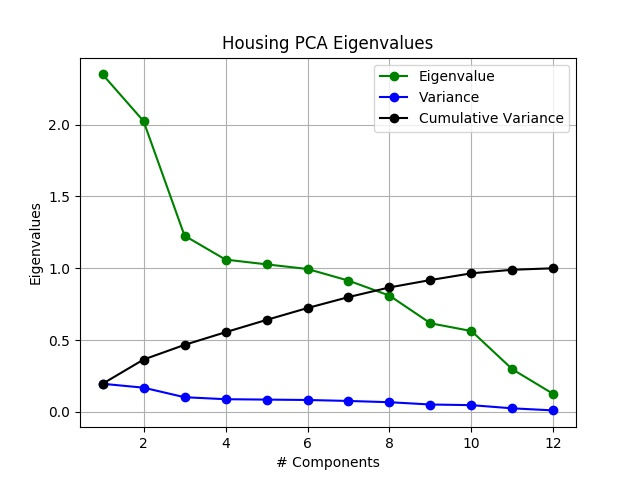
\includegraphics[width=1\textwidth,keepaspectratio]{housing_pca_eigenvalues.jpg} 
      \caption*{Housing Principal Components Analysis } 
   \endminipage\hfill
\end{figure}

\subsubsection*{Analysis}
IText

\subsection*{2) Independent Components Analysis (ICA)}  
\subsubsection*{Overview}
Text

 \begin{figure}[H]
  \minipage{0.49\textwidth}
      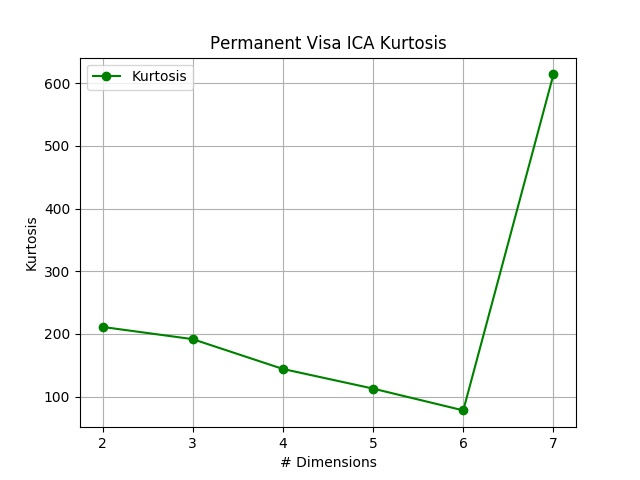
\includegraphics[width=1\textwidth,keepaspectratio]{permanent_visa_ica_kurtosis.jpg} 
      \caption*{Permanent Visa Independent Components Analysis } 
   \endminipage\hfill
    \minipage{0.49\textwidth}
      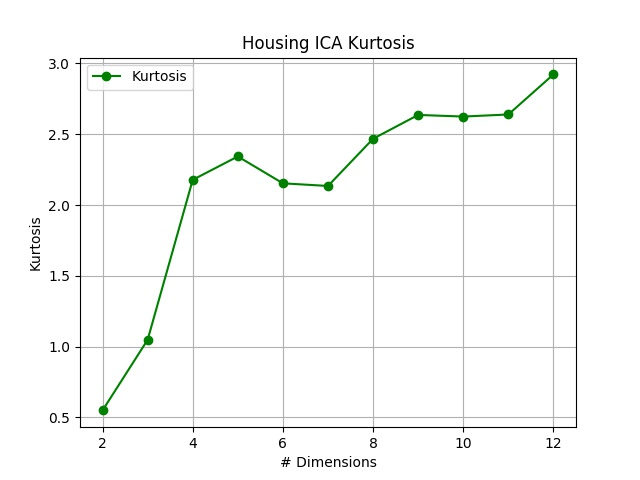
\includegraphics[width=1\textwidth,keepaspectratio]{housing_ica_kurtosis.jpg} 
      \caption*{Housing Independent Components Analysis } 
   \endminipage\hfill
\end{figure}


\subsubsection*{Analysis}
IText

\subsection*{3) Randomized Projections}  
\subsubsection*{Overview}
Text

 \begin{figure}[H]
  \minipage{0.49\textwidth}
      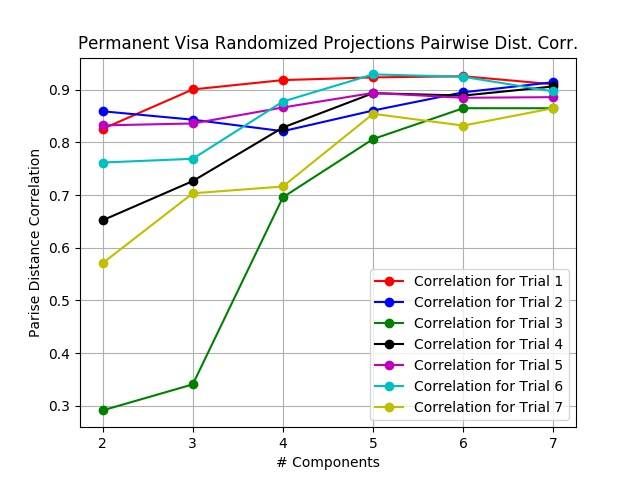
\includegraphics[width=1\textwidth,keepaspectratio]{permanent_visa_randomized_projections_pairwise_distpt_corrpt.jpg} 
      \caption*{Permanent Visa Randomized Projections Pairwise Correlation } 
   \endminipage\hfill
    \minipage{0.49\textwidth}
      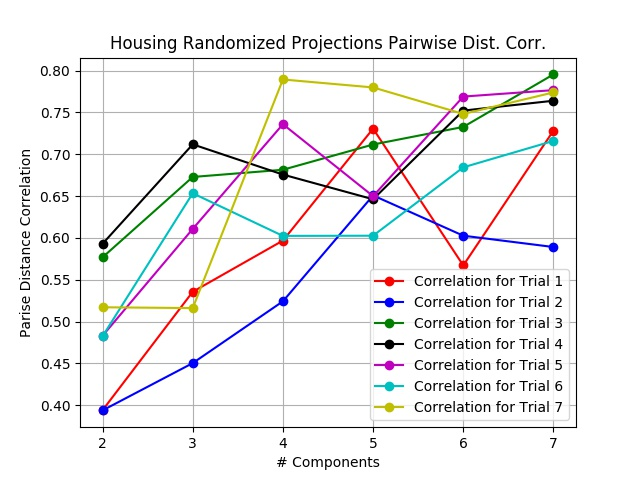
\includegraphics[width=1\textwidth,keepaspectratio]{housing_randomized_projections_pairwise_distpt_corrpt.jpg} 
      \caption*{Housing Randomized Projections Pairwise Correlation} 
   \endminipage\hfill
\end{figure}
 \begin{figure}[H]
  \minipage{0.49\textwidth}
      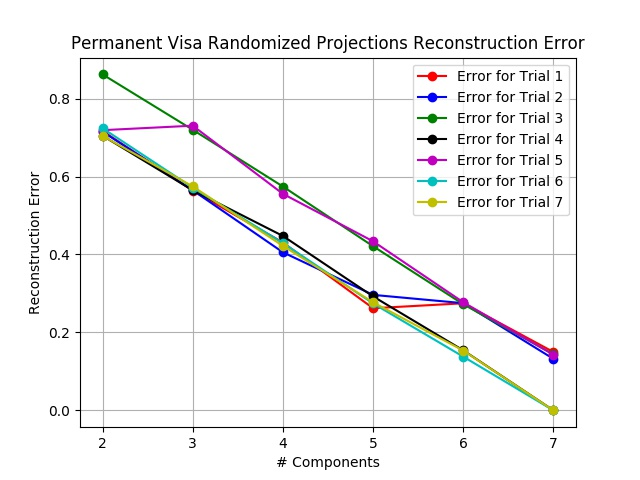
\includegraphics[width=1\textwidth,keepaspectratio]{permanent_visa_randomized_projections_reconstruction_error.jpg} 
      \caption*{Permanent Visa Randomized Projections Reconstruction Error } 
   \endminipage\hfill
    \minipage{0.49\textwidth}
      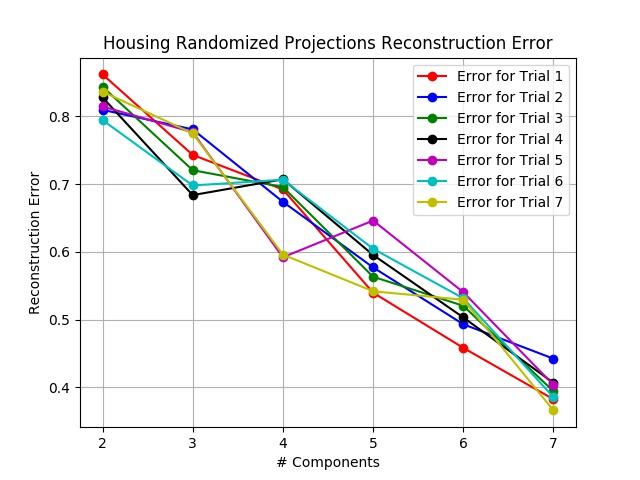
\includegraphics[width=1\textwidth,keepaspectratio]{housing_randomized_projections_reconstruction_error.jpg} 
      \caption*{Housing Randomized Projections Reconstruction Error} 
   \endminipage\hfill
\end{figure}

\subsubsection*{Analysis}
IText

\subsection*{4) Random Forests}  
\subsubsection*{Overview}
Text

 \begin{figure}[H]
  \minipage{0.49\textwidth}
      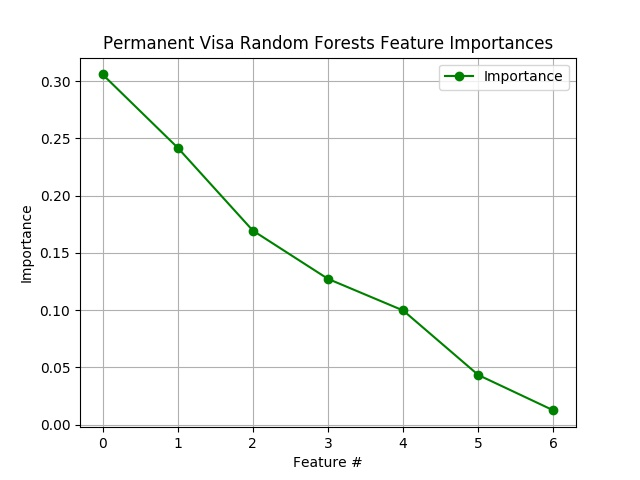
\includegraphics[width=1\textwidth,keepaspectratio]{permanent_visa_random_forests_feature_importances.jpg} 
      \caption*{Permanent Visa Random Forest Feature Importances (Descending Order) } 
   \endminipage\hfill
    \minipage{0.49\textwidth}
      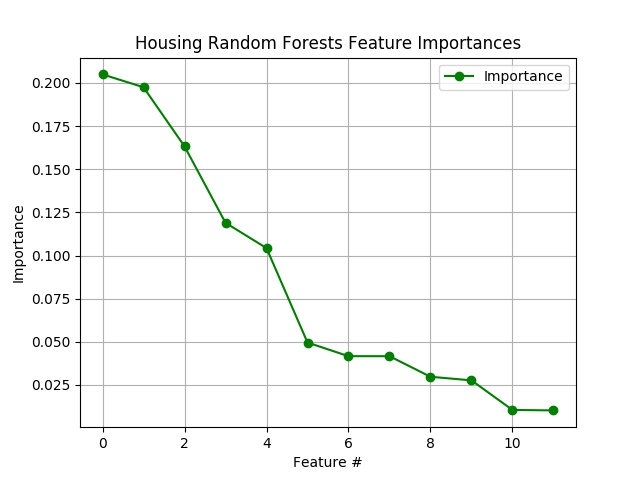
\includegraphics[width=1\textwidth,keepaspectratio]{housing_random_forests_feature_importances.jpg} 
      \caption*{Housing Random Forest Feature Importances (Descending Order)} 
   \endminipage\hfill
\end{figure}

\subsubsection*{Analysis}
IText


\section*{Conclusion}  
Todo conclusion

\end{document}